\section{Qualitative Beobachtung verschiedener Kreiselbewegung}
Bei diesem Teil des Versuches wurde ein nutationsfreier Kreisel beobachtet. Es wurde bei verschiedenen Drehzahlen mit dem Finger Kräfte auf die Figurenachse ausgeübt. Es wurde zwei Fälle betrachtet.\\\\
\textbf{1. Fall: keine Kraftausübung}
\begin{itemize}
\item Zuerst wurde der Kreisel auf die entsprechende niedrige Frequenz gebracht (ca. \(f=1,1\,\text{Hz}\)) und anschließend ohne den Einsatz von äußeren Einflüssen, d.h. es wurde keine zusätzliche Kraft auf hin ausgeübt, beobachtet. Der Kreisel rotierte wie erwartet und man konnte lediglich die Rotationsachse sehen. Die Rotationsachse fällt mit der Figurenachse zusammen, sie können nicht voneinander unterschieden werden.
\item Nun wurde die Frequenz erhöht. Die ungefähr eingestellte Drehfrequenz betrug in etwa \\\(f=25\,\text{Hz}\). Auch hier wurde quantitativ beobachtet, dass die Drehimpulsachse, Figurenachse und die Rotationsachse übereinander lagen.
\end{itemize}
\textbf{2. Fall: geringe Kraftausübung}
\begin{itemize}  
\item Der Kreisel wurde wieder auf die niedrig Drehfrequenz gebracht. Diesmal wurde jedoch auf den Kreisel eine Kraft ausgeübt. Bei leichter Kraftausübung mit dem Finger konnte man beobachten, dass der Kreisel versucht dieser Kraft entgegenzuwirken. Wenn diese Kraft nun senkrecht zur Drehachse ausgeübt wurde, kam es zur einer leichten Präzessionsbewegung. Wie bereits in den Fragen zur Vorbereitung diskutiert (\ref{sec:Praezession}), präzediert ein Kreisel immer in die Richtung des Drehimpulses, dies wurde auch bei dem Versuch beobachtet. Die ausgeübte Kraft lenkte die Figurenachse aus, woraufhin sich diese Achse in die selbe Richtung bewegt, wie der Drehimpuls.  
\item Es wurde auch hier die Drehfrequenz erhöht. Hier kam es auch zur einer Präzessionsbewegung, allerdings war diese hier stärker ausgeprägt. Aber qualitativ wurde beobachtet, dass auch hier der Kreisel in Richtung des Drehimpulses präzediert.
\end{itemize}
\newpage
Als nächstes wurde nun die Nutation genauer beobachtet. Nutation ruft man hervor, indem man den Kreisel mit einer Stange einen Schlag  versetzt, dadurch trennen sich die Figurenachse, Drehimpulsvektor und momentane Drehachse voneinander.
\begin{itemize}
\item Zuerst wurde die Nutation ohne Stoboskop beobachtet. Wenn man nun von oben auf den rotierenden Kreisel sieht, kann man einen formstabilen Punkt erkennen, der eine Kreisbewegung ausführt. Auf dem Kreisel sind 3 verschiedene Farben angebracht, somit erkennt man das der Punkt die Farbe "wechselt". Zur Verdeutlichung wird das in Abbildung \ref{img:Nutation} schematisch dargestellt. 
\begin{figure}[h]
\begin{center}
	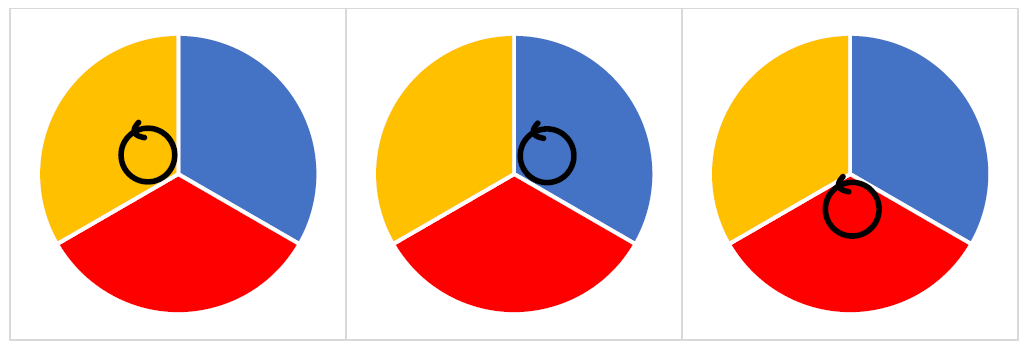
\includegraphics[width=8cm]{nutation.png}
	\caption{Schematische Darstellung der Nutation}
	\label{img:Nutation}
\end{center}
\end{figure}

\item Als letztes wurde der Kreisel noch mit dem Stroboskop beleuchtet. Das Stroboskoplicht wurde auf die Drehfrequenz des Kreisels eingestellt. So erkennt man, dass die Gewindestange eine Kegelförmige Bewegung ausführt und somit einen Nutationskegel bildet. Zur genaueren Erläuterung wurde während dem Versuch ein Bild aufgenommen und der entstehende Kegel nach skizziert, dies ist in der folgenden Abbildung \ref{img:belichtung} zu erkennen. 
\begin{figure}[h]
\begin{center}
	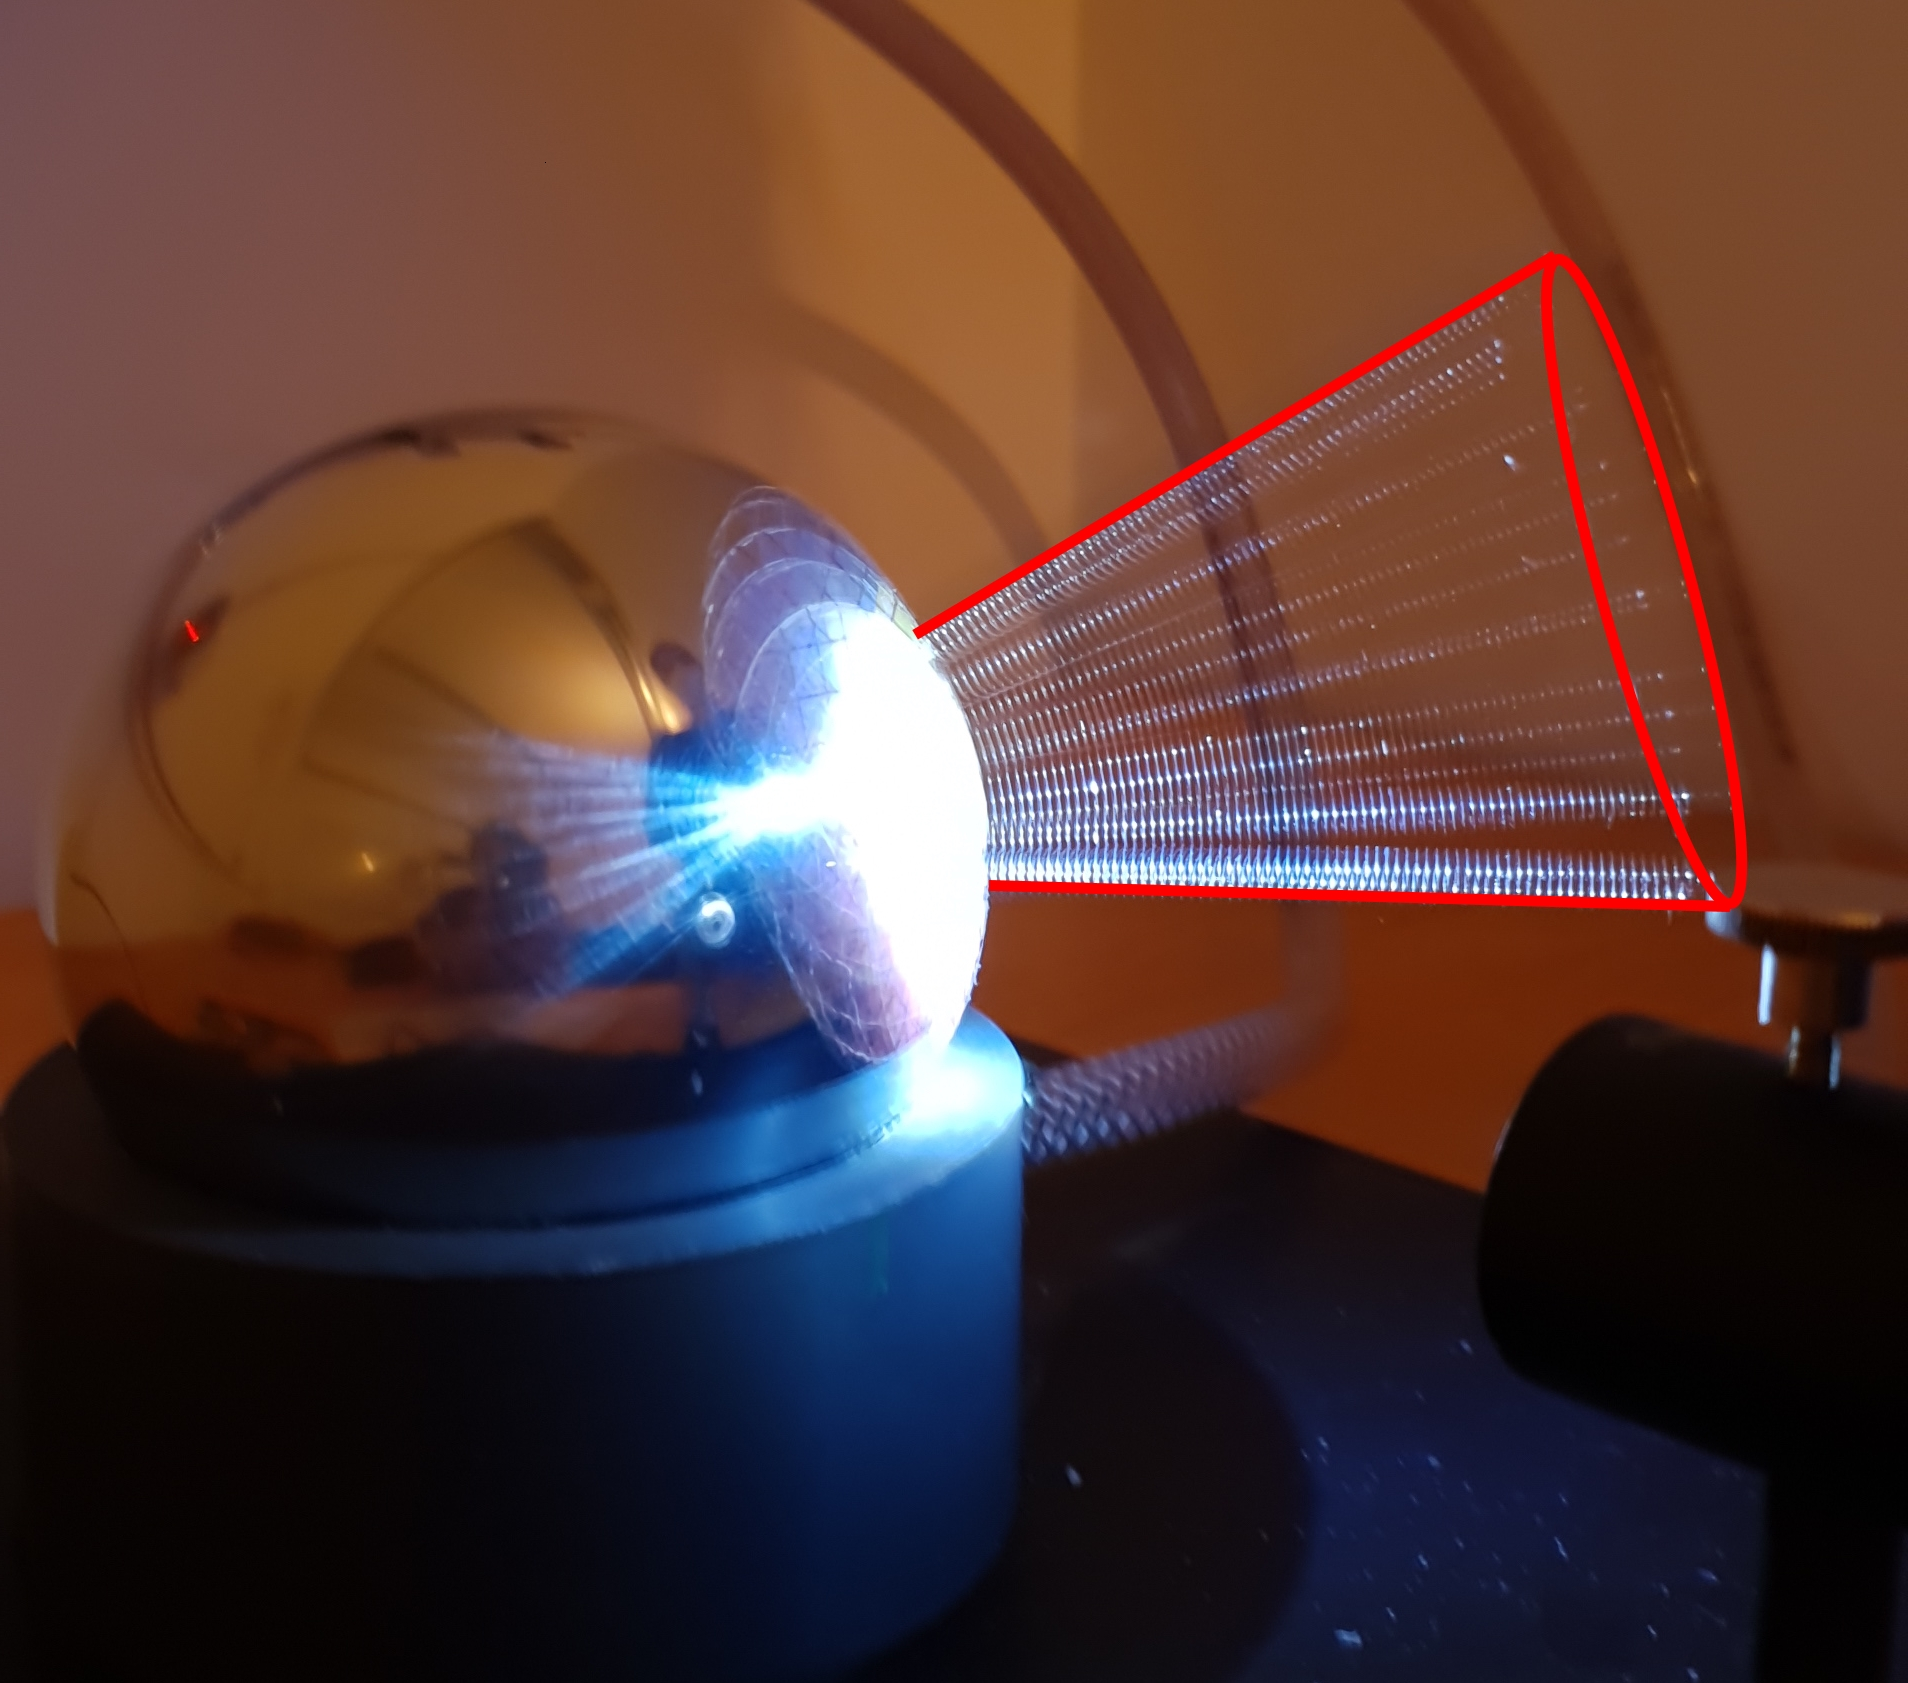
\includegraphics[width=8cm]{belichtung_ink}
	\caption{Schematische Darstellung der Nutation}
	\label{img:belichtung}
\end{center}
\end{figure}

\end{itemize}




